\chapter{Metodologia}

\section{Aparato experimental e combustível}
O protótipo de reator disponibilizado pela Koala Energy consiste em um reator de dois estágios, um de volatilização (inferior) e outro de combustão (superior). O ar atmosférico é injetado no reator por um ventilador centrífugo da fabricante ebm-papst, sendo que, ao entrar no reator, o fluxo de ar se divide em dois: um é direcionado ao fundo do reator, onde passa pela grelha e pela cama de pellets, proporcionando as condições para a gaseificação da biomassa (referido daqui em diante como injeção primária de ar); o segundo fluxo é dirigido aos orifícios na parede interna do queimador, localizados no topo (injeção secundária de ar). Esse último fluxo proporcionará a combustão dos gases gerados no fundo do reator, completando o processo.

Um desenho simplificado do reator é mostrado na Figura \ref{fig:queimador_koala}. O orifício lateral maior é onde há a conexão com o ventilador. A circulação do ar destinado à injeção secundária no interior da parede do reator é vantajosa, tendo em vista que o ar é pré-aquecido nesse processo. Entretanto, o dispositivo não conta com um mecanismo de regulagem de vazão especificamente para as injeções primária e secundária. 

\begin{figure}[!ht]
	\centering
	\caption{Modelo do queimador usado no presente estudo.}
	\frame{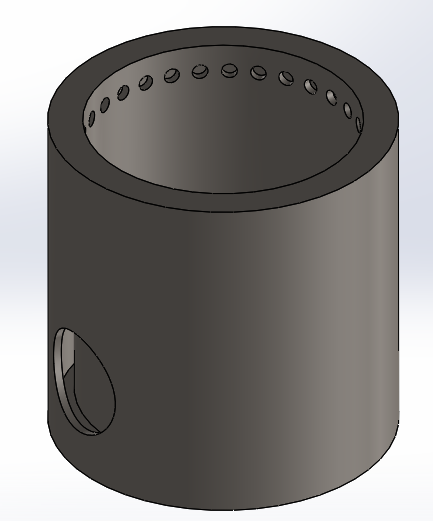
\includegraphics[scale=0.5]{Textuais/experimental/vista_opaca.png}}
	\frame{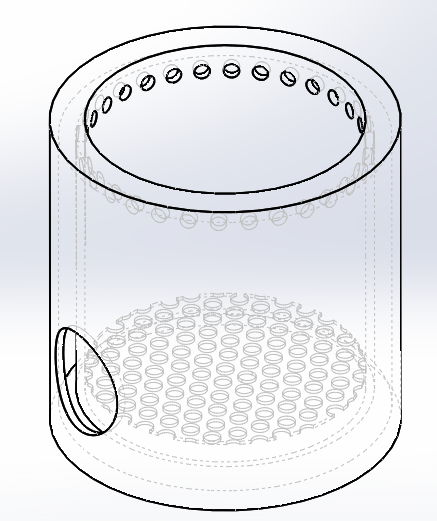
\includegraphics[scale=0.5]{Textuais/experimental/vista_transparente.png}}
	\fonte{O autor (2022).}
	\label{fig:queimador_koala}
\end{figure}

Para permitir um estudo mais completo, a empresa projetou e fabricou um sistema de alimentação automático de combustível, além de uma capela para exaustão de gases. Também foi disponibilizado o sistema de controle elétrico, por meio do qual é possível controlar a vazão de combustível, o acionamento do ventilador do queimador e o sistema de exaustão da capela. O aparato experimental disponibilizado pela empresa é mostrado na Figura \ref{fig:aparatokoala} (imagem obtida antes de serem iniciados os testes).

\begin{figure}
	\centering
	\caption{Aparato experimental disponibilizado pela empresa.}
	\frame{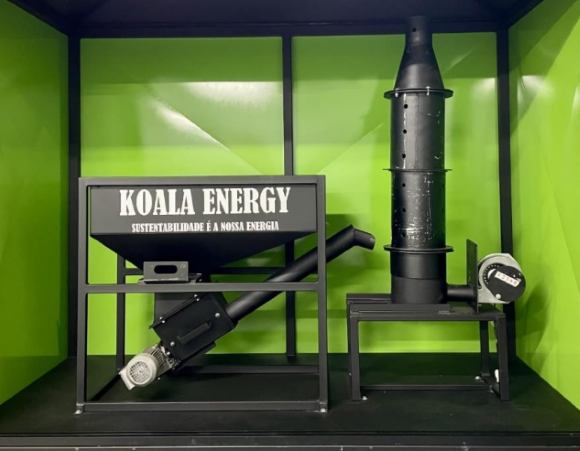
\includegraphics[scale=0.5]{Textuais/experimental/capela.png}}
	\fonte{O autor (2022).}
	\label{fig:aparatokoala}
\end{figure}

O combustível utilizado são pellets de madeira do gênero \textit{pinus}, proveniente de reflorestamento, sendo produzidos a partir de resíduos da indústria de processamento de madeira. O produto possui certificação \textit{ENplus} A1, o mais alto nível na classificação da \textit{ENplus}, órgão de origem europeia voltado a certificação de pellets. A avaliação do instituto é feita com base nas normas ISO, levando em conta as variáveis associadas ao combustível. Na Figura \ref{fig:pellets_koala} são mostrados os pellets produzidos pela empresa.

\begin{figure}[!ht]
	\centering
	\caption{Pellets produzidos pela empresa Koala Energy.}
	\frame{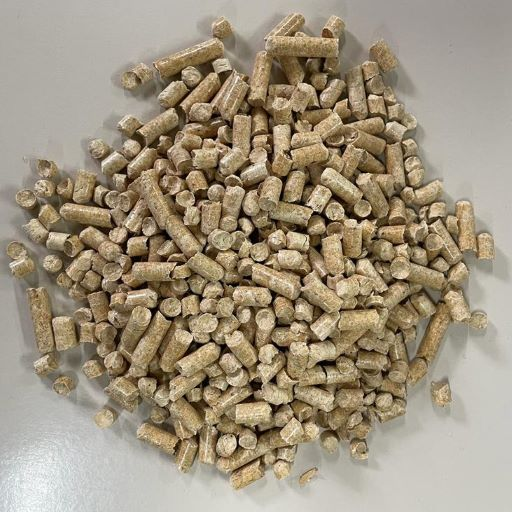
\includegraphics[scale=0.5]{Textuais/experimental/pellets_koala.jpeg}}
	\fonte{O autor (2022).}
	\label{fig:pellets_koala}
\end{figure}

Alguns parâmetros importantes dos pellets, fornecidos pela empresa, são mostrados na Tabela \ref{tab:propriedadespellets}.

\begin{table}[!ht]
	\centering
	\small
	\renewcommand{\arraystretch}{1.3}
	\caption{Algumas propriedades dos pellets da Koala, informados pela empresa.}%
	\label{tab:propriedadespellets}
        \begin{tabular}{|l|c|}
        \hline
        \multicolumn{1}{|c|}{\textbf{Propriedade}} & \textbf{Valor} \\ \hline
        Diâmetro                                   & 6,6 mm         \\ \hline
        Densidade aparente                         & 720 kg/m³      \\ \hline
        Teor de cinzas (a 550°C, bs)               & 0,5\%          \\ \hline
        \multirow{2}{*}{PCI} & 5,11 kWh/kg    \\ \cline{2-2} 
                                                   & 18,40 MJ/kg    \\ \hline
        Teor de enxofre (bs)                       & 0,014\%        \\ \hline
        Teor de nitrogênio (bs)                    & 0,16\%         \\ \hline
        \end{tabular}
	\vspace{2mm}
	\fonte{O autor (2022).}
\end{table}

Outra análise relevante em relação ao combustível é a análise elementar, usada para modelar matematicamente a reação, como será visto adiante. Tendo em vista não ser possível realizar essa análise no Centro de Ciências Tecnológicas da Udesc, não foi possível obter essa análise em tempo hábil para os ensaios. Portanto, foi usada a composição elementar de outra biomassa semelhante como base. A análise escolhida foi a de Neves et al. (2017), anteriormente mostrada na Tabela \ref{tab:elementar}, e novamente na Tabela \ref{tab:elementar_modelagem}. Nesta Tabela, $Y$ representa a fração mássica de cada elemento. 

\begin{table}[!ht]
	\centering
	\small
	\renewcommand{\arraystretch}{1.3}
	\caption{Composição elementar dos pellets usada para obter o modelo matemático.}%
	\label{tab:elementar_modelagem}
        \begin{tabular}{|l|l|l|l|l|l|l|}
        \hline
        \textbf{Elemento} & C    & H   & O    & N   & S & Cinzas \\ \hline
        \textbf{Y (\%)}   & 49,1 & 6,6 & 43,5 & 0,1 & - & 0,7    \\ \hline
        \end{tabular}
	\vspace{2mm}
	\fonte{Adaptada de Neves et al. (2017).}
\end{table}


\section{Variáveis medidas}

\subsection{Temperatura e emissão de poluentes}
Para caracterizar o processo de combustão dos gases gerados no processo de volatilização, as principais métricas necessárias são o perfil de temperatura e emissão de poluentes. Dessa forma, é necessário um dispositivo que permita acoplar os instrumentos de medição ao processo. O dispositivo projetado no laboratório foi uma chaminé, dividida em 3 seções, que possui função tanto no monitoramento da temperatura quanto na avaliação dos poluentes. A representação 3D do conjunto é mostrada na Figura \ref{fig:projeto_chamine}.

\begin{figure}
	\centering
	\caption{Projeto da chaminé para medição de temperatura e emissões.}
	\frame{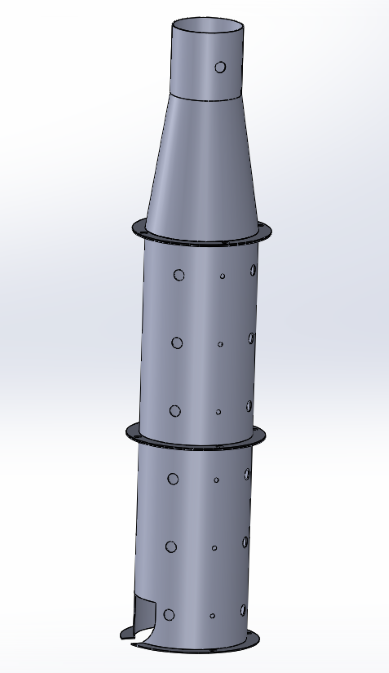
\includegraphics[scale=0.5]{Textuais/experimental/projeto_chamine.png}}
	\fonte{O autor (2022).}
	\label{fig:projeto_chamine}
\end{figure}

A primeira seção (de baixo para cima) possui uma abertura lateral para permitir que o alimentador de pellets seja posicionado corretamente. Os orifícios maiores possibilitam o posicionamento da sonda de gases, enquanto os orifícios menores permitem a inserção dos termopares. O segundo estágio possui função idêntica ao primeiro, enquanto o terceiro permite unicamente a medição de poluentes. Esse último estágio possui um perfil cônico, que permite uma uniformização do fluxo de gases, permitindo uma medição de poluentes final mais adequada. Antes dos testes, a chaminé foi revestida com uma manta térmica de fibra cerâmica, visando reduzir a perda de calor pelas paredes.

Os termopares utilizados são do tipo K, sendo possível posicioná-los a uma distância inicial de 50 mm do reator e após em intervalos regulares de 100 mm entre si. No presente estudo a medição de temperatura foi feita somente em um ponto, sendo o termopar posicionado no orifício de medição de temperatura mais alto da chaminé. O termopar foi conectado ao sistema de aquisição de dados Keysight (Figura \ref{fig:keysight}), que por sua vez é conectado a um computador, permitindo monitorar a temperatura através do software Keysight BenchVue.

\begin{figure}[!ht]
	\centering
	\caption{Sistema de aquisição de dados Keysight e software BenchVue.}
	\frame{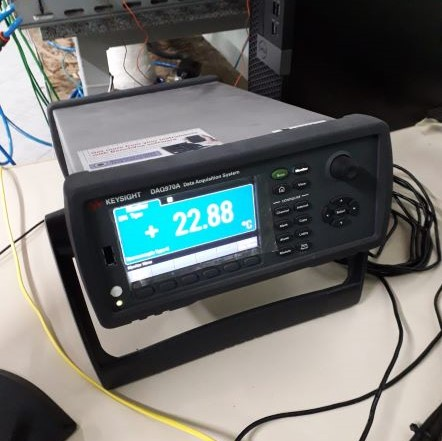
\includegraphics[scale=0.5]{Textuais/experimental/keysight.jpeg}}
	\frame{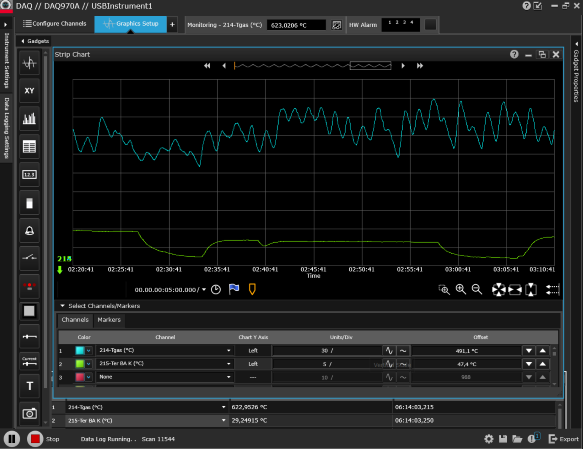
\includegraphics[scale=0.49]{Textuais/experimental/keysightbenchvue.png}}
	\fonte{O autor (2022).}
	\label{fig:keysight}
\end{figure}

O equipamento para medição de poluentes utilizado foi o Testo 350 (Figura \ref{fig:testo}), que conta com uma sonda que pode ser posicionada em cada um dos furos maiores da chaminé. O equipamento fornece dados de concentração de \ch{CO}, $\ch{NO}_x$, \ch{CO2}, \ch{O2} e hidrocarbonetos para um dado combustível, ajustado no equipamento previamente às medições. Todas as medições foram realizadas no topo da chaminé, posicionando-se a sonda no orifício logo acima ao perfil cônico.

\begin{figure}
	\centering
	\caption{Analisador de gases Testo 350.}
	\frame{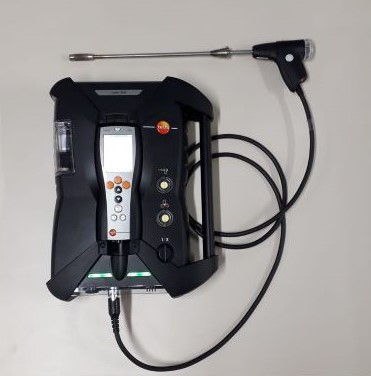
\includegraphics[scale=0.6]{Textuais/experimental/testo.jpeg}}
	\fonte{O autor (2022).}
	\label{fig:testo}
\end{figure}

\subsection{Vazão de combustível}
Os pellets de madeira são despejados no reator através de um sistema de alimentação, composto de um silo e um parafuso, acoplado a um motor elétrico trifásico. O motor é conectado a um controlador lógico programável (CLP), que permite ajustar os parâmetros relativos ao fornecimento de combustível. Esses parâmetros são:

\begin{enumerate}[noitemsep,nosep,labelindent=\parindent,leftmargin=*,label={\alph*})] 
	\item Tempo de descarga inicial: tempo em que a rosca despeja os pellets que serão usados na ignição do reator;
	\item Tempo de aguardo inicial: tempo entre a descarga de combustível inicial e o início do funcionamento do reator no modo automático;
	\item Tempo do ventilador: tempo para o qual o ventilador liga, a partir da descarga inicial;
	\item Tempo de descarga ($TH$): tempo no qual a rosca despeja pellets no reator, em modo automático;
	\item Tempo de aguardo ($TL$): intervalo de tempo entre as descargas de combustível, em modo automático.
\end{enumerate}

Os três primeiros parâmetros listados possuem função apenas no acendimento do reator, enquanto os dois últimos são fundamentais na análise do sistema operando em regime permanente. Nesse caso, é possível determinar a vazão mássica de combustível (Equação \eqref{eq:mdotpellet}) sabendo-se qual a massa de pellets despejada no tempo $TH$ ($m_{pellet} (TH)$) e o tempo de um ciclo ($T_{ciclo} = TL + TH$).
\begin{equation} \label{eq:mdotpellet}
\dot{m}_{comb} = \frac{m_{pellet} (TH)}{TL + TH}.
\end{equation}

O parâmetro $m_{pellet}(TH)$ médio foi determinado experimentalmente para diferentes tempos $TH$. O número de amostras $N$ necessário para a obtenção de uma média cujo desvio padrão populacional fosse $\sigma$, confiabilidade fosse $z$ e precisão fosse $L$, foi calculado com base na Equação \eqref{eq:ene}.
\begin{equation} \label{eq:ene}
N = \frac{z\sigma}{L}.
\end{equation}

O parâmetro $\sigma$ foi estimado a partir de 31 medições para $TL = 0,5$ s, número de medições para o qual pode-se usar o teorema do limite central \cite{Devore}. Para um parâmetro $z$ correspondente à 95\% de confiabilidade e precisão $L$ de 2 g, o número de amostras necessário foi $N=26$. A massa de pellets em cada amostra foi avaliada com uma balança de precisão Shimadzu, de resolução 0,01 g. A Tabela \ref{tab:mdot} relaciona os valores obtidos.

\begin{table}[!ht]
	\centering
	\small
	\renewcommand{\arraystretch}{1.3}
	\caption{Massa de combustível média fornecida ao reator para diferentes tempos de descarga.}%
	\label{tab:mdot}
        \begin{tabular}{|c|c|}
        \hline
        $TH$ (s) & $m_{pellet}(TH)$ (g)    \\ \hline
        0,1    & 10,87                     \\ \hline
        0,5    & 49,98                     \\ \hline
        1      & 96,22                     \\ \hline
        2      & 191,50                    \\ \hline
        \end{tabular}
    \vspace{2mm}
	\fonte{O autor (2022).}
\end{table}

\subsection{Vazão de ar}
%A vazão de ar é determinada usando-se um anemômetro de fio quente da fabricante Testo GmbH, modelo 445. Para uma melhor segurança em relação aos valores medidos, foi realizada uma aferição do equipamento em relação aos valores registrados, com o auxílio de uma câmara de teste de fluxo de ar da fabricante Airflow. A câmara conta com dois conjuntos de bocais, uma com 3 bocais de diâmetro externo 4 in e outra com 4 bocais, de diâmetros 2 in, 1,6 in, 1 in e 0,688 in. Um dos conjuntos é posicionado no centro da câmara e o outro na extremidade de saída. No momento em que o ar passa pelos bocais no centro do equipamento, existe uma queda na pressão do fluido, que é aferida com base em duas tomadas de pressão conectadas ao equipamento. Com a pressão manométrica sendo registrada por um manômetro de coluna de água Dwyer, e sendo conhecido o diâmetro dos bocais, é possível determinar a vazão de ar, através de cartas fornecidas pelo fabricante da câmara. Sabendo-se a vazão de ar e o diâmetro do bocal externo, é possível determinar a velocidade do ar teórica de maneira direta, tendo em vista que o bocal uniformiza o escoamento (i.e. a velocidade ao longo da seção transversal do bocal não varia), através da equação \eqref{eq:vazao}.
%\begin{equation} \label{eq:vazao}
%Q = V\cdot A.
%\end{equation}

%\noindent Essa velocidade, considerada como a teórica, é comparada com a velocidade registrada pelo anemômetro, que foi posicionado na saída do bocal. O procedimento foi realizado para 10 velocidades do ar, situadas no intervalo de 0 a 10 m/s. Para atingir essas velocidades, o bocal posicionado no centro do equipamento é o de 2 in, e na saída o de 4 in. A curva mostrada na Figura \ref{fig:curva} foi obtida.

%\begin{figure}
%	\centering
%	\caption{Curva de calibração obtida para o anemômetro.}
%	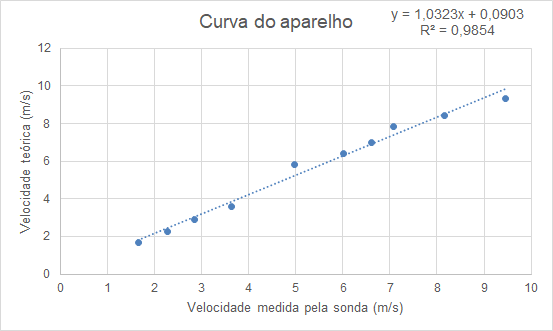
\includegraphics[scale=0.8]{Textuais/curva_calibracao_testo.png}
%	\fonte{O autor.}
%	\label{fig:curva}
%\end{figure}

O aparato experimental construído para medição da vazão consiste nos itens relacionados na lista abaixo. Uma visão geral do aparato experimental é mostrada na Figura \ref{fig:aparato}.
\begin{enumerate}[noitemsep,nosep,labelindent=\parindent,leftmargin=*,label={\alph*}) ] 
	\item Um bocal cônico para separação de fluxos de ar;
	\item Um tubo de PVC, de 75 mm de diâmetro nominal e 2,18 m de comprimento;
	\item Um tubo de Pitot, com ajuste de altura;
	\item Um manômetro de coluna de precisão da marca Dwyer.
\end{enumerate}

\begin{figure}[!ht]
	\centering
	\caption{Aparato experimental construído para medição da vazão.}
	\frame{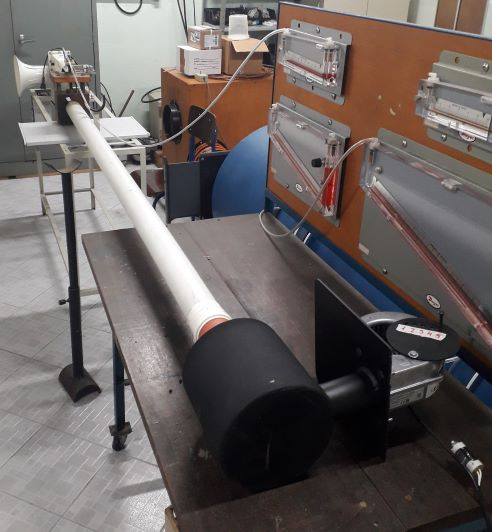
\includegraphics[scale=0.4]{Textuais/experimental/aparato.jpg}}
	\fonte{O autor (2022).}
	\label{fig:aparato}
\end{figure}

Vale ressaltar que as medições foram realizadas com o reator na horizontal, o que não influencia o resultado final. A medição da vazão de ar foi realizada em duas etapas: a primeira medição serviu para determinar somente a vazão da injeção primária, enquanto a segunda determinou a vazão total de ar (incluindo a injeção secundária). Para tanto foi usado o bocal cônico, como mostrado na Figura \ref{fig:cone}.

\begin{figure}[!ht]
	\centering
	\caption{Cone para separação dos fluxos de ar do fundo e das laterais.}
	\frame{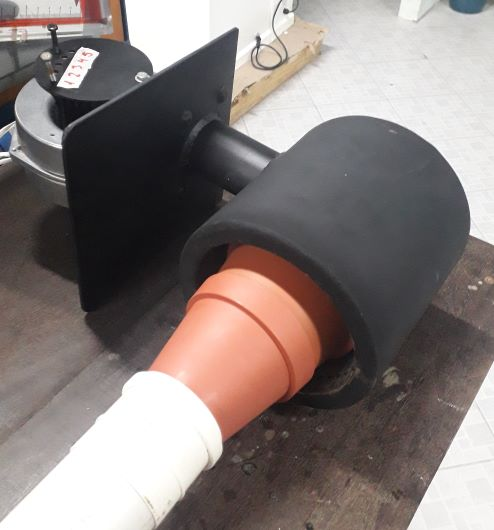
\includegraphics[scale=0.4]{Textuais/experimental/bottom.jpg}}
	\fonte{O autor (2022).}
	\label{fig:cone}
\end{figure}

O cone pode ser fixo em qualquer ponto ao longo da parede interna do reator. Portanto, para determinar a vazão proveniente do fundo do reator, o dispositivo foi fixado abaixo dos orifícios laterais, cuidando-se para que não haja obstrução desses (como é mostrado na Figura \ref{fig:cone}). Já para a medição da vazão total, o cone foi posicionado logo acima dos orifícios. Ao cone foi acoplado o tubo de PVC, que possui comprimento suficiente para permitir que o escoamento se torne completamente desenvolvido. O material do tubo possui rugosidade baixa, de forma que os efeitos de perda de carga não foram considerados.

A vazão de ar ar fornecida pelo ventilador acoplado ao queimador foi determinada considerando-se as 5 posições de ajuste da abertura de ar (Figura \ref{fig:posicoes}), convencionando-se a posição 1 para vazão máxima e a posição 5 para vazão mínima.

\begin{figure}[!ht]
	\centering
	\caption{Posições de abertura do ventilador.}
	\frame{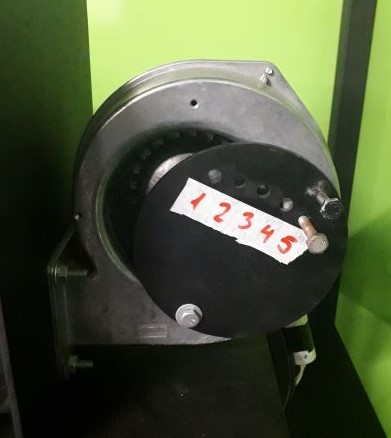
\includegraphics[scale=0.4]{Textuais/experimental/posicoes.jpg}}
	\fonte{O autor (2022).}
	\label{fig:posicoes}
\end{figure}

Para determinar a vazão de ar deve-se primeiramente obter a velocidade média do escoamento, que depende do regime desse (laminar ou turbulento). O regime de um escoamento interno em um tubo é avaliado pelo número de Reynolds relativo ao diâmetro, $Re_{D}$, Equação \eqref{eq:reynolds}.
\begin{equation} \label{eq:reynolds}
Re_D = \frac{VD}{\nu}.
\end{equation}

No caso de a quantia ser avaliada na posição de velocidade máxima do escoamento (linha central do tubo), $V = U$ e a notação é modificada para $Re_{U}$. Considerando a viscosidade cinemática do ar a 25°C na pressão atmosférica como $\nu = 1,5\cdot 10^{-5} m^2/s$ com base em dados de Fox (1998), espera-se um regime turbulento, de forma que não existe uma relação universal entre o campo de tensões e o campo de velocidade média \cite{Fox}. Uma das abordagens é usar um perfil experimental, sendo um dos mais usados o perfil de lei de potência, da forma da Equação \eqref{eq:perfil}.
\begin{equation} \label{eq:perfil}
\frac{\bar{u}}{U} = {\left(\frac{y}{R}\right)}^{1/n}.
\end{equation}

\noindent A coordenada $y$ possui origem na parede do tubo, sendo que para cada valor dessa coordenada é possível determinar uma velocidade média temporal $\bar{u}$ no ponto. O termo $n$ é determinado por correlações experimentais; Hinze apud Fox (1998) sugere que, para um escoamento interno em tubo liso, o expoente pode ser determinado pela Equação \eqref{eq:nturbulento}. 
\begin{equation} \label{eq:nturbulento}
n = -1,7 + 1,8\cdot log(Re_U).
\end{equation}

Na prática, o perfil previsto pela Equação \eqref{eq:perfil} pode ser avaliado com um tubo de Pitot, dispositivo com o qual é possível medir a variação da pressão de um escoamento em determinado ponto e então determinar a velocidade desse. O tubo de Pitot do aparato experimental conta com uma regulagem de altura, que permite medir a velocidade do escoamento ao longo do diâmetro do tubo. Um paquímetro também é acoplado, para permitir a medição do comprimento em relação à parede do tubo. A pressão obtida pelo tubo de Pitot é avaliada com base em um manômetro de coluna de água da fabricante Dwyer, com escala de 1 polegada de água ($in_{\ch{H2O}})$ e resolução de 0,01 $in_{\ch{H2O}}$. Ambos os dispositivos são mostrados na Figura \ref{fig:pitot}.

\begin{figure}[!ht]
	\centering
	\caption{Tubo de Pitot e manômetro de coluna de líquido.}
	\frame{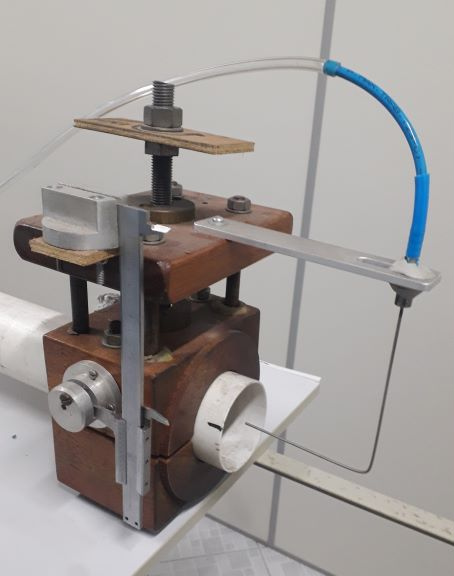
\includegraphics[scale=0.31]{Textuais/experimental/pitot_mini.jpg}}
	\frame{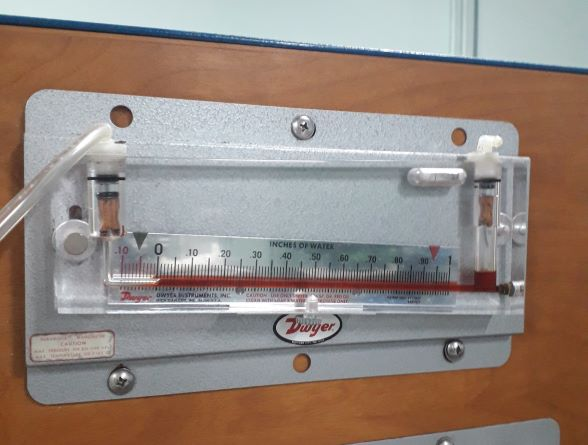
\includegraphics[scale=0.4]{Textuais/experimental/barometro.jpg}}
	\fonte{O autor (2022).}
	\label{fig:pitot}
\end{figure}

O tubo de Pitot fornece a pressão de estagnação $P_{0}$ do escoamento. Além dessa pressão, é necessário conhecer a pressão estática $P$. Como pode ser observado na Figura \ref{fig:pitot}, a ponta do tubo foi posicionada exatamente alinhada com o final do tubo de PVC, de forma que $P$ fio considerada a pressão atmosférica. Definindo a diferença de pressão como $\Delta P = P_{0} - P$, a velocidade do escoamento em qualquer posição ao longo do diâmetro do tubo pode ser determinada a partir da definição de pressão dinâmica, dando origem à Equação \eqref{eq:pitot}. O uso dessa expressão requer que o tubo esteja alinhado na horizontal, caso no qual a variação de energia potencial do escoamento pode ser desprezada. Dessa forma, o duto de PVC foi cuidadosamente alinhado na horizontal, com o auxílio de um nível.
\begin{equation} \label{eq:pitot}
V = \sqrt{\frac{2\Delta P}{\rho_{ar}}}.
\end{equation}

Assim, para verificar se o perfil de velocidade proposto por Hinze modela convenientemente o fenômeno, foi realizado um teste onde a pressão estática foi medida em vários pontos ao longo do diâmetro do tubo, visando a obtenção de um perfil de velocidade para uma vazão fixa. O valores de velocidade em função da posição obtidos são denotados pelos pontos azuis na Figura \ref{fig:vteoexp}, onde o sistema de coordenadas y possui origem na parede do tubo e termina na linha de centro. Com base no número de Reynolds da velocidade na linha de centro $Re_{U}$ foi determinado o expoente $n$ para essa velocidade, e com isso foi possível determinar um perfil de velocidade da forma da Equação \eqref{eq:perfil}, denotado pela linha vermelha na Figura \ref{fig:vteoexp}.

\begin{figure}[!ht]
	\centering
	\caption{Pontos experimentais e perfil de velocidade previsto pela Equação \eqref{eq:perfil}}.
	\frame{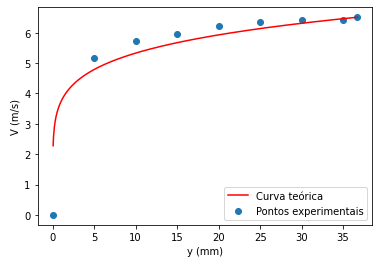
\includegraphics[scale=0.8]{Textuais/experimental/vteoexp.png}}
	\fonte{O autor (2022).}
	\label{fig:vteoexp}
\end{figure}

Como observado pelo gráfico, a curva traçada com base na Equação \eqref{eq:perfil} apresentou-se próxima às velocidades experimentais obtidas para cada ponto, sendo que o erro máximo verificado entre os pontos experimentais foi de 7,67\%, em y = 10 mm. Destaca-se que o perfil teórico não descreve bem o comportamento próximo à parede (para valores de $y/R < 0,04$), e não possui inclinação nula no centro, fato que pode ser observado no gráfico; todavia, são erros inerentes ao modelo \cite{Fox}. Devido à simplicidade matemática e boa aproximação do comportamento real, o modelo de perfil de potência será usado, permitindo o uso das Equações \eqref{eq:nturbulento} e \eqref{eq:vsobreu}. 

Para determinar a vazão volumétrica, é necessário determinar a velocidade média do escoamento ($\bar{V}$), a qual pode ser estimada com base na medição experimental da velocidade apenas na linha de centro ($U$) e no expoente $n$, conforme apresentado pela Equação \eqref{eq:vsobreu}, obtida por meio da integração da Equação \eqref{eq:perfil}.
\begin{equation} \label{eq:vsobreu}
\frac{\bar{V}}{U} = \frac{2n^{2}}{(n+1)(2n+1)}.
\end{equation}

\noindent Sendo conhecida $\bar{V}$, a vazão volumétrica pode ser determinada pela Equação \eqref{eq:vazaovol}.
\begin{equation} \label{eq:vazaovol}
{Q} = {\bar{V}} \cdot A_{tr}.
\end{equation}
\noindent O termo $A_{tr}$ representa a área da seção transversal do tubo, cujo diâmetro é de 70
mm. Dessa forma, o procedimento experimental consistiu nas seguintes etapas:




\begin{enumerate}[noitemsep,nosep,labelindent=\parindent,leftmargin=*,label={\alph*}) ] 
	\item Medição da velocidade no centro do tubo utilizando-se o tubo de Pitot;
	\item Determinação da velocidade média do escoamento ($\bar{V}$) por meio da Equação \eqref{eq:vsobreu};
	\item Determinação da vazão volumétrica ($Q$).
\end{enumerate}

A partir dos procedimentos descritos, as vazões volumétricas foram medidas e estão apresentadas na Tabela \ref{tab:vazoes}, sendo os valores apresentados em $m^3/s$ e litros por minuto (LPM).

\begin{table}[!ht]
	\centering
	\small
	\renewcommand{\arraystretch}{1.3}
	\caption{Vazões volumétricas obtidas para as 5 posições de abertura do ventilador.}%
	\label{tab:vazoes}
        \begin{tabular}{|c|cc|cc|cc|}
        \hline
        \multirow{2}{*}{Posição} & \multicolumn{2}{c|}{Injeção primária} & \multicolumn{2}{c|}{Total}            & \multicolumn{2}{c|}{Injeção secundária} \\ \cline{2-7} 
                         & \multicolumn{1}{c|}{m³/s}    & LPM    & \multicolumn{1}{c|}{m³/s}    & LPM    & \multicolumn{1}{c|}{m³/s}      & LPM    \\ \hline
        1                        & \multicolumn{1}{c|}{0,0222}  & 1332,0 & \multicolumn{1}{c|}{0,03517} & 2110,2 & \multicolumn{1}{c|}{0,01292}   & 775,2  \\ \hline
        2                        & \multicolumn{1}{c|}{0,0221}  & 1326,0 & \multicolumn{1}{c|}{0,03466} & 2079,6 & \multicolumn{1}{c|}{0,01253}   & 751,8  \\ \hline
        3                        & \multicolumn{1}{c|}{0,0219}  & 1314,0 & \multicolumn{1}{c|}{0,03356} & 2013,6 & \multicolumn{1}{c|}{0,01165}   & 699,0  \\ \hline
        4                        & \multicolumn{1}{c|}{0,0210}  & 1260,0 & \multicolumn{1}{c|}{0,03281} & 1968,6 & \multicolumn{1}{c|}{0,01181}   & 708,6  \\ \hline
        5                        & \multicolumn{1}{c|}{0,0193}  & 1158,0 & \multicolumn{1}{c|}{0,03044} & 1826,4 & \multicolumn{1}{c|}{0,01114}   & 668,4  \\ \hline
        \end{tabular}
	\vspace{2mm}
	\fonte{O autor.}
\end{table}

Pode-se observar que a posição de abertura da placa posicionada na entrada no ventilador resultou na variação da vazão de ar total em torno de 13\%. Ainda, a vazão na injeção secundária representa cerca de 36\% da vazão total para todas as posições de abertura do ventilador.

Um teste preliminar do queimador em operação foi realizado a fim de determinar se as vazões de ar obtidas permitem um funcionamento adequado do queimador. Para uma injeção de combustível de 1 s a cada 40 s, para a menor vazão de ar (posição 5), verificou-se uma chama muito intensa, como pode ser verificado na Figura \ref{fig:preliminar}. Essa chama inviabilizaria as medições, principalmente da emissão de poluentes.

\begin{figure}[!ht]
	\centering
	\caption{Teste preliminar do queimador com a vazão de ar de 1826,4 LPM (posição 5).}
	\frame{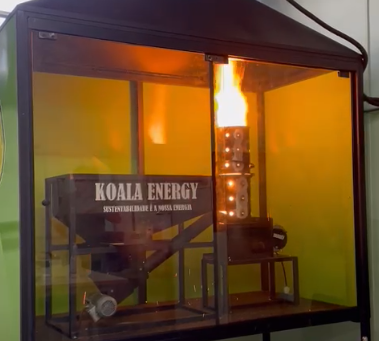
\includegraphics[scale=0.8]{Textuais/experimental/preliminar.png}}
	\fonte{O autor (2022).}
	\label{fig:preliminar}
\end{figure}

Assim, buscou-se por um mecanismo que pudesse diminuir a vazão volumétrica de ar. Optou-se por uma placa de orifícios, que permite reduzir o fluxo de ar sem a necessidade de ajustar características elétricas do ventilador. Além disso, foram feitos mais dois orifícios na placa de controle de vazão, permitindo o ajuste de mais duas posições da placa, que permite mais dois valores de vazão (inferores aos já existentes). Esses orifícios foram nomeados 6 e 7, respectivamente. Para registrar as novas vazões volumétricas o procedimento adotado, bem como as equações utilizadas, foram idênticos ao caso anterior. Entretanto, as pressões registradas através do tubo de Pitot eram muito baixas, de forma que para uma medição mais precisa de velocidade foi usado um anemômetro de fio quente, da fabricante Testo GmbH, modelo 445. O anemômetro foi posicionado na extremidade do tubo, no centro desse em relação à seção transversal, na posição onde anteriormente estava o tubo de Pitot, como mostra a Figura \ref{fig:fioquente}. As novas vazões obtidas são mostradas na Tabela \ref{tab:vazoesnova}.

\begin{figure}[!ht]
	\centering
	\caption{Posicionamento do anemômetro de fio quente.}
	\frame{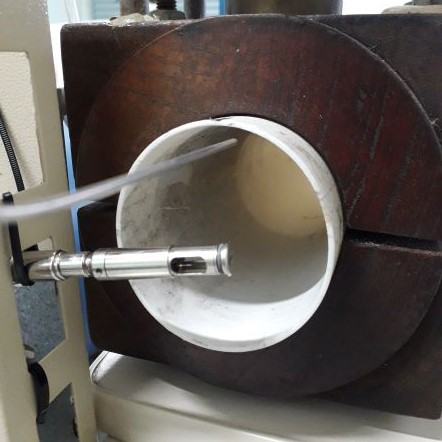
\includegraphics[scale=0.4]{Textuais/experimental/fiquente.jpg}}
	\fonte{O autor (2022).}
	\label{fig:fioquente}
\end{figure}


\begin{table}[!htbp]
	\centering
	\small
	\renewcommand{\arraystretch}{1.3}
	\caption{Novas vazões volumétricas medidas.}%
	\label{tab:vazoesnova}
        \begin{tabular}{|c|cc|cc|cc|}
        \hline
        \multirow{2}{*}{Posição} & \multicolumn{2}{c|}{Injeção primária} & \multicolumn{2}{c|}{Total}           & \multicolumn{2}{c|}{Injeção secundária} \\ \cline{2-7} 
                                 & \multicolumn{1}{c|}{m³/s}     & LPM   & \multicolumn{1}{c|}{m³/s}    & LPM   & \multicolumn{1}{c|}{m³/s}      & LPM    \\ \hline
        1                        & \multicolumn{1}{c|}{0,00239}  & 143,4 & \multicolumn{1}{c|}{0,00478} & 286,5 & \multicolumn{1}{c|}{0,00239}   & 143,2  \\ \hline
        2                        & \multicolumn{1}{c|}{0,00232}  & 139,4 & \multicolumn{1}{c|}{0,00461} & 276,4 & \multicolumn{1}{c|}{0,00228}   & 137,0  \\ \hline
        3                        & \multicolumn{1}{c|}{0,00226}  & 135,4 & \multicolumn{1}{c|}{0,00454} & 272,3 & \multicolumn{1}{c|}{0,00228}   & 136,9  \\ \hline
        4                        & \multicolumn{1}{c|}{0,00222}  & 133,4 & \multicolumn{1}{c|}{0,00437} & 262,2 & \multicolumn{1}{c|}{0,00215}   & 128,7  \\ \hline
        5                        & \multicolumn{1}{c|}{0,00209}  & 125,5 & \multicolumn{1}{c|}{0,00420} & 252,0 & \multicolumn{1}{c|}{0,00211}   & 126,6  \\ \hline
        6                        & \multicolumn{1}{c|}{0,00196}  & 117,5 & \multicolumn{1}{c|}{0,00403} & 241,9 & \multicolumn{1}{c|}{0,00207}   & 124,4  \\ \hline
        7                        & \multicolumn{1}{c|}{0,00179}  & 107,6 & \multicolumn{1}{c|}{0,00383} & 229,8 & \multicolumn{1}{c|}{0,00204}   & 122,1  \\ \hline
        \end{tabular}
	\vspace{2mm}
	\fonte{O autor (2022).}
\end{table}

Verifica-se que a proporção de 36\% estimada pelos testes iniciais não se manteve, sendo alterada para valores próximos de 50\%. Ou seja, a quantidade de ar destinada aos processos de volatilização e oxidação é aproximadamente igual.


\section{Parâmetros de operação como função das variáveis medidas}
Para determinar os parâmetros de operação do queimador de acordo com os parâmetros iniciais, foi elaborado um código computacional no software EES (Engineering Equation Solver). A fim de determinar uma expressão para a razão de equivalência ($\Phi$), é necessário inicialmente conhecer a fração combustível-ar estequiométrica ($F_s$), obtida pela equação química da reação global que ocorre com o pellet. Tendo em vista que os pellets possuem um teor de enxofre usualmente desprezível, a Equação química \eqref{eq:combestbio} se reduz a Equação \eqref{eq:combpellet}.
\begin{equation} \label{eq:combpellet}
\ch{C} \ch{H}_a \ch{O}_b \ch{N}_c + a_t(\ch{O2} + 3,76 \ch{N2}) \rightarrow{} x \ch{CO2} + y \ch{H2O} + w \ch{N2}.
\end{equation}

\noindent A reação pode ser reescrita em base molar, sendo cada componente do combustível especificado separadamente. 
\begin{equation} \label{eq:combpelletn}
n_c \ch{C} + n_H \ch{H} + n_O \ch{O} + n_N \ch{N} + a_t(\ch{O2} + 3,76 \ch{N2}) \rightarrow{} x \ch{CO2} + y \ch{H2O} + w \ch{N2}.
\end{equation}

\noindent Na Equação \eqref{eq:combpelletn} $n_i$ é definido como segue. $MW_i$ é a massa molar de cada componente, e as frações $Y_i$ são obtidas da Tabela \ref{tab:elementar_modelagem}.
\begin{equation} \label{eq:enee}
n_i = \frac{Y_i}{MW_i}.
\end{equation}
% em kmol/kgcomb

Aplicando-se a conservação da massa para cada espécie química:
\begin{enumerate}[noitemsep,nosep,labelindent=\parindent,leftmargin=*,label={\alph*}) ] 
	\item Balanço de \ch{C}:
	\begin{equation}
	    x = n_C.    
	\end{equation}
	\item Balanço de \ch{H}:
	\begin{equation}
	    n_H = 2y.    
	\end{equation}
    \item Balanço de \ch{O}:
	\begin{equation}
	    n_O + a_t = 2x + y.    
	\end{equation}
    \item Balanço de \ch{N}:
	\begin{equation}
	    a_t\cdot3,76\cdot2 = 2w.    
	\end{equation}
\end{enumerate}

\noindent O termo $F_s$, considerando-se a combustão completa de 1 kg de combustível, é dada pela Equação \eqref{eq:Fs}. A massa molecular do ar foi determinada a 25°C e 1 atm diretamente através do EES.
\begin{equation} \label{eq:Fs}
F_s = \frac{n_C\cdot MW_C + n_H\cdot MW_H + n_O\cdot MW_O + n_N\cdot MW_N}{4,76\cdot a_t \cdot MW_{ar}}.
\end{equation}

\noindent Em termos dos dados fornecidos, a fração combustível-ar $F$ é dada por:
\begin{equation} \label{eq:F}
F = \frac{\dot{m}_{comb}}{\dot{m}_{ar}}
\end{equation}

\noindent onde o termo $\dot{m}_{comb}$ é dado pela Equação \eqref{eq:mdotpellet} e $\dot{m}_{ar}$ provém da Tabela \ref{tab:vazoesnova}, bastando-se apenas converter os valores de vazão total de $m^3/s$ para $kg/s$ através da densidade do ar $\rho_{ar}$, avaliada a 25°C e 1 atm.
\begin{equation} \label{eq:VtoM}
\dot{m}_{ar} \left[\frac{kg}{s}\right]= {Q}_{ar} \left[\frac{m^3}{s}\right] \cdot \rho_{ar} \left[\frac{kg}{m^3}\right]
\end{equation}

As Equações \eqref{eq:VtoM}, \eqref{eq:F}, \eqref{eq:Fs}, \eqref{eq:mdotpellet}, \eqref{eq:Pot} e \eqref{eq:phi} foram reunidas no código computacional. Para determinar os parâmetros de operação do queimador, é necessário somente informar três variáveis iniciais; para os testes realizados, foram informados os valores da vazão volumétrica de ar total ${Q}_{ar}$, razão de equivalência $\Phi$ desejada e tempo de despejo $TH$. O EES permite a construção de tabelas paramétricas, de forma que os dados foram arranjados nesse modelo, como mostrado pela Figura \ref{fig:tabparam}. 

\begin{figure}[!ht]
	\centering
	\caption{Exemplo de tabela paramétrica do EES.}
	\frame{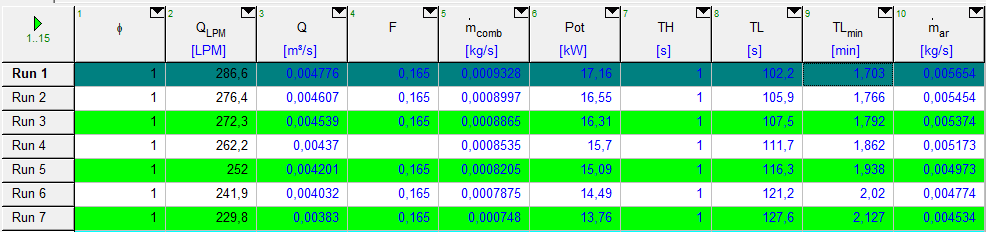
\includegraphics[scale=0.6]{Textuais/experimental/tabela_EES.png}}
	\fonte{O autor (2022).}
	\label{fig:tabparam}
\end{figure}

\section{Execução dos testes}
Os testes consistiram em avaliações quantitativas e qualitativas do processo de combustão no reator, com o sistema operando em regime automático (com alimentações de combustível periódicas). O primeiro teste consistiu na verificação do comportamento da chama e das condições de operação do reator para $\Phi = 1$ em 4 potências, avaliando de maneira visual a intensidade da chama e a estabilização das reações ao longo do tempo. Da mesma forma, o segundo conjunto de testes consistiu na mesma avaliação para $\Phi = 0,7$, dessa vez para 3 potências. As imagens para determinar o perfil da chama foram registradas a uma distância padronizada do queimador. Os testes qualitativos permitiram uma validação preliminar do aparato experimental, permitindo ajustes importantes antes do início das medições. A partir dos primeiros testes também foi possível determinar os melhores parâmetros para acendimento do reator, sendo eles:

\begin{enumerate}[noitemsep,nosep,labelindent=\parindent,leftmargin=*,label={\alph*})] 
	\item Tempo de descarga inicial: 5 segundos;
	\item Tempo de aguardo inicial: 7 minutos;
	\item Tempo do ventilador: 4 minutos (após o tempo de descarga inicial);
\end{enumerate}

O terceiro conjunto de testes consistiu propriamente na medição de temperatura e emissão de poluentes do queimador. Nesses testes foi usada a chaminé, já devidamente isolada, sendo um teste realizado para $\Phi = 1$ e três testes para $\Phi = 0,7$. O perfil de temperatura obtido para todos os testes foi oscilatório, como já esperado inicialmente, tendo em vista o fato da alimentação ser intermitente. Dessa forma, para determinar se o sistema estava em regime permanente, foi verificada a amplitude do perfil de temperatura; se esse intervalo se mostrava dentro de uma mesma faixa de temperatura por aproximadamente 20 minutos, o processo era considerado em regime permanente. Após a estabilização, foram realizadas as medições de emissão de poluentes, sendo a sonda posicionada no orifício de medição superior da chaminé por aproximadamente 7 minutos, sendo 2 minutos necessários para estabilização dessas medições. O processo é mostrado na Figura \ref{fig:eu}.

\begin{figure}[!t]
	\centering
	\caption{Medição de poluentes sendo realizada.}
	\frame{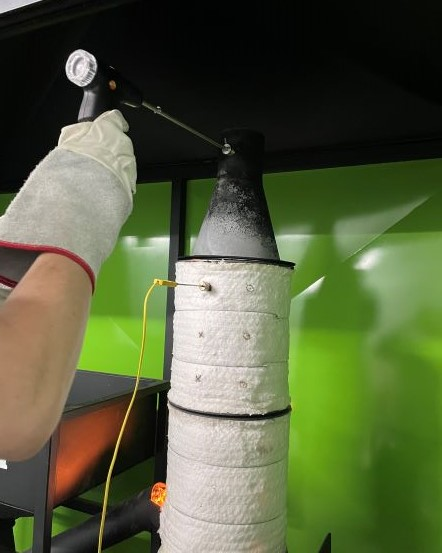
\includegraphics[scale=0.5]{Textuais/results/medindo.jpeg}}
	\fonte{O autor (2022).}
	\label{fig:eu}
\end{figure}


% \section{Infos adicionais}
% Medidas experimentais do diâmetro do queimador:

% $d_1 = 20,35 cm$

% $d_2 = 20,3 cm$

% $d_3 = 20,28 cm$

% $d_4 = 20,38 cm$

% $d_5 = 20,3 cm$

% Vídeos de queimadores semelhantes:

% https://www.youtube.com/watch?v=kvRK0lC1UKk

% https://www.youtube.com/watch?v=5Oxm-sO39MM

% https://www.youtube.com/watch?v=4OqJTvxrdLw

% Testes que podem ser realizados:

% - Fixar vazão mássica e ver o comportamento em 5 vazões de ar distintas (estimar phi para cada caso)

% - Determinar a potência máxima 

% - Emissão de poluentes (provavelmente somente para a menor vazão, pra não danificar o testo): CO, NOx, CO2

% - Distribuição de temperaturas (se possível)

% Coisas pra fazer

% - Fotos sem o tubo de Pitot

